\documentclass[12pt, a4paper]{article}

\usepackage[a4paper,top=3cm,bottom=3cm,left=3cm,right=3cm]{geometry}
\usepackage[T1]{fontenc}
\usepackage{graphicx}
\graphicspath{{figures/}}
\usepackage{caption}
\usepackage{subcaption}
\usepackage{hyperref}
\usepackage{float}
\usepackage{amsmath}

\hypersetup{
	colorlinks=true,
	linkcolor=black,
	filecolor=magenta,
	urlcolor=cyan,
}

\begin{document}
\thispagestyle{empty}

\begin{center}
	{\bfseries \LARGE Reinforcement Learning \\[2mm]
	Mini-Project-2}

	\vfill

	{\large
	\textbf{Pielat Krystian} \\[2mm]
	\textbf{Sangineto Marina} \\[2mm]
	\textbf{Sauvenay Antoine}
	}

	\vfill

	%
\includegraphics[width=0.35\textwidth]{plots/sorbonne.png}

	\vfill

	{\large Sorbonne Université} \\[2mm]
	{\large 2025}
\end{center}

\newpage
\tableofcontents
\newpage

\section{Introduction}

In this project, we use the BBRL framework to study the effects of partial observability on the continuous-action version of the \textit{LunarLander-v3} environment and \textit{CartPoleContinuous-v1} environment with the TD3 algorithm.\\

To simulate partial observability, we implemented dedicated env wrappers. We investigate if extending the input to the agent’s policy and critic with a memory of previous states helps to combat the challenges of partial observability. Additionally, we explore the impact of using action chunks(sequences of consecutive actions) rather than single-step actions, achieved through temporal extension wrappers.\\

The study focuses on a single performance metric: the mean reward. The goal of the trained algorithms is to maximize it. Both environments have different arbitrary reward calculation rules. In \textit{LunarLander-v3}, the agent controls a lander using continuous main and side thrusters to land softly on a designated pad. Reward increases as the lander approaches the pad, maintains upright orientation, and lands gently, while penalties apply for speed, tilt, or fuel use. Crashes give large negative rewards, and successful landings give large bonuses. In \textit{CartPoleContinuous-v1}, the agent applies continuous horizontal force to keep a pole balanced upright on a moving cart. The reward is +1 for every timestep the pole remains balanced within bounds, ending when the pole falls or the cart moves too far.


\section{Wrappers}

The \texttt{FeatureFilterWrapper} removes a specific feature from the returned observation during calls to the \texttt{reset()} and \texttt{step(action)} functions. The feature to be removed is specified as an index when constructing the wrapper object.

For example, to filter out the x and y velocities of the lander in the LunarLander-v3 environment, the wrapper can be applied multiple times as follows:
\[
\texttt{env = FeatureFilterWrapper(FeatureFilterWrapper(inner\_env, X), Y)}
\]
where \texttt{inner\_env} refers to the environment, and \texttt{X} and \texttt{Y} represent the indices of the features to be filtered out.

\subsection{Exercise 1: Implementing the \texttt{FeatureFilterWrapper} Class}

The purpose of the \texttt{FeatureFilterWrapper} is to simulate partial observability by removing selected features from the observation vector. This allows evaluating TD3’s robustness with incomplete state information. The wrapper modifies the \texttt{reset()} and \texttt{step(action)} functions to filter out specified features before returning observations. 

\subsection{Exercise 2: Implementing the \texttt{ObsTimeExtensionWrapper} Class}

The \texttt{ObsTimeExtensionWrapper} provides the agent with short-term memory by concatenating the current observation with the previous observation. This temporal extension allows the agent to infer velocity and acceleration information that may have been removed by partial observability. The implementation maintains a \texttt{previous\_obs} buffer initialized with zeros during \texttt{reset()} and updated after each \texttt{step()}. 

\subsection{Exercise 3: Implementing the \texttt{ActionTimeExtensionWrapper} Class}

The \texttt{ActionTimeExtensionWrapper} modifies the action space by requiring the agent to output a sequence of $M$ consecutive actions at each decision step, but only the first action is executed by the environment. 



\section{Experimental Study}

In this section presents the experimental study comparing TD3 performance under various observability conditions and temporal extension configurations.

\subsection{Architectural Choices}

For this exercise, the TD3 (Twin Delayed Deep Deterministic Policy Gradient) algorithm was used in the continuous version of the \textit{LunarLander-v3} environment, as required. We decided to additionally run the experiments on the \textit{CartPoleContinuous-v1} environment and tune new set of hyperparameters for it. TD3 is characterized by its robustness and stability in continuous control problems, relying on twin critics, delayed policy updates, and target smoothing to reduce overestimation bias.\newline

For exploration, we employed Ornstein–Uhlenbeck noise using the \texttt{AddOUNoise} agent. This temporally correlated noise model is particularly suitable for continuous control tasks, as it produces smoother exploration trajectories compared to uncorrelated Gaussian noise. \newline

We initially attempted to optimize the model hyperparameters in each environment using \textit{Optuna}. However, due to the high computational cost of the training process, we decided to resign from full quantitative hyperparameter optimization and instead tuned the parameters empirically by testing multiple configurations and comparing their performance in TensorBoard.

\subsection{Experimental Setup}

To systematically evaluate the impact of partial observability and temporal extensions, we designed four experimental configurations:

\begin{enumerate}
	\item \textbf{Baseline / Full observability}: Full observability with the original 8-dimensional observation space of LunarLander-v3. This serves as the reference performance level.

	\item \textbf{Partial Observability}: Removed the horizontal and vertical velocities ($\dot{x}$ and $\dot{y}$) using two nested \texttt{FeatureFilterWrapper} instances, reducing the observation space.

	\item \textbf{Observation Memory}: Applied \texttt{ObsTimeExtensionWrapper} to the baseline environment, expanding the observation space by concatenating current and previous observations.

	\item \textbf{Action Chunking}: Applied \texttt{ActionTimeExtensionWrapper} with sequence length $M=3$, expanding the action space from 2 to 6 dimensions. Only the first action in each sequence is executed, promoting temporal consistency in the policy.
	
\end{enumerate}


Apart from these main configurations, we also tested several combined setups to evaluate how \textit{observation memory} and \textit{action chunking} could mitigate the loss of information caused by partial observability.

Each configuration was trained for 1000 episodes using 5 random seeds (1-5) to ensure statistical robustness. All experiments used identical TD3 hyperparameters (different set for LunarLander and different for CartPole, they can be found \href{https://github.com/KrystianPielat/rl-project-2/blob/master/run_experiments.py}{here}).

\subsection{Results and Analysis}

\begin{figure}[H]
	\centering
	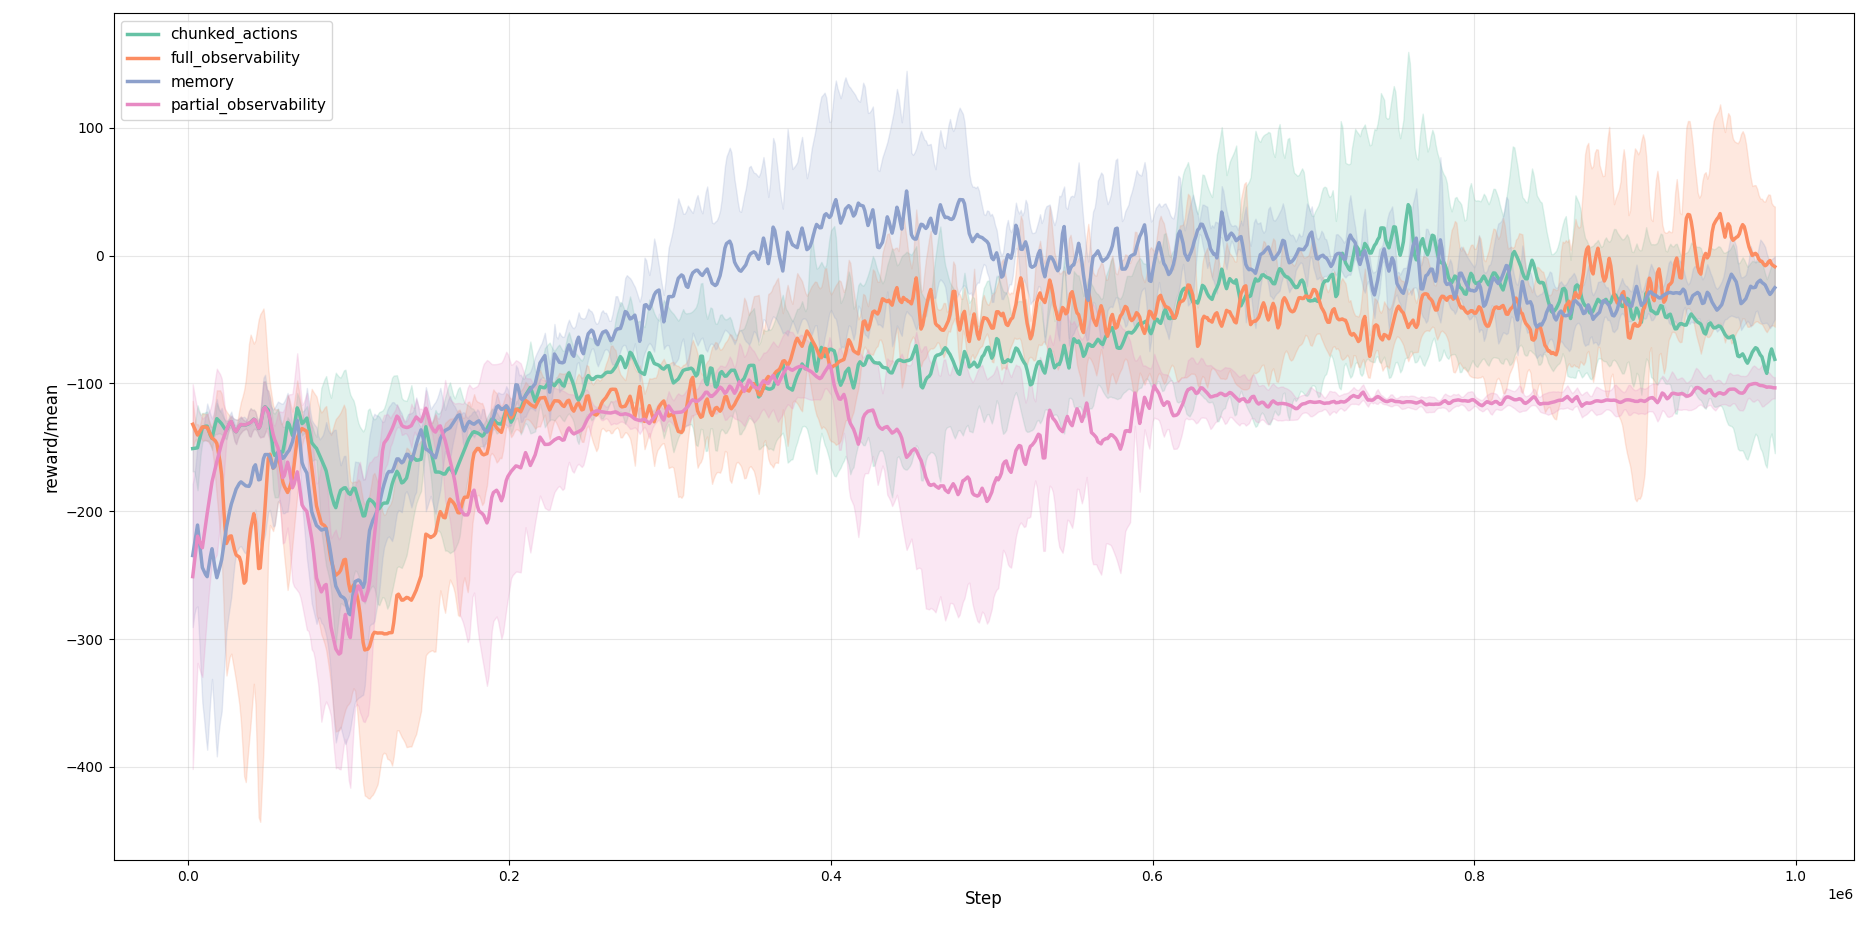
\includegraphics[width=1\linewidth]{results_lunar_lander_basic}
	\caption{Results without combining wrappers.}
	\label{fig:resultslunarlanderbasic}
\end{figure}

\begin{figure}[H]
	\centering
	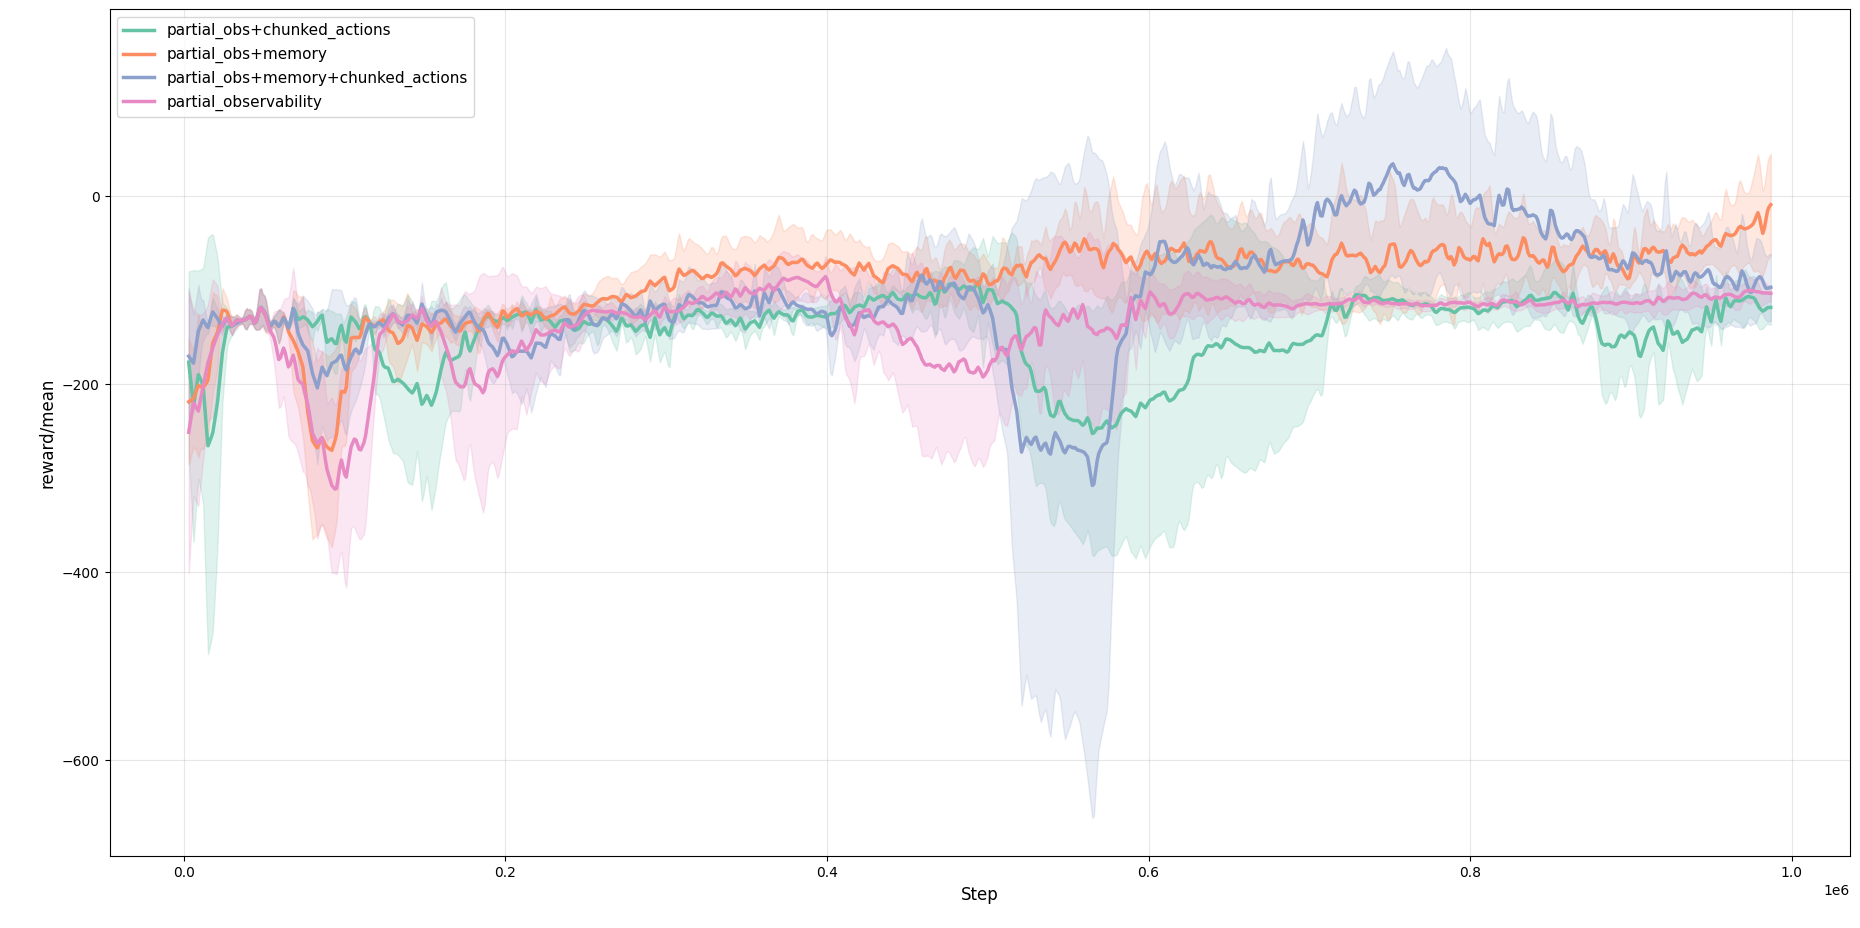
\includegraphics[width=1\linewidth]{results_lunar_lander_combined}
	\caption{Results of partial observability configurations combined with other wrappers.}
	\label{fig:resultslunarlandercombined}
\end{figure}


\subsubsection{General Results}

Based on figure \ref{fig:resultslunarlanderbasic} all algorithms demonstrated stable learning and consistent improvement. The results would be more insightful if they were ran on more than 5 seeds per configuration (more precise confidence intervals) and with more training steps, however our study was limited by computational resources.

The performance of the baseline configuration with full observability was approximately in the middle between the other configurations, which aligns with intuition, given it was neither hindered by removing information about the environment, nor improved by providing additional information like memory.

\subsubsection{Partial Observability}
When horizontal and vertical velocities were removed (\textit{partial\_observability} configuration), we see on figure \ref{fig:resultslunarlanderbasic} that performance degradation was  observable. The agent struggled more during training, slower convergence and plateauing around lower average reward than other algorithms. This confirms that velocity information is critical for optimal landing control - without it, the agent must rely on position changes across timesteps to estimate velocities, which introduces noise and delays in control responses.

\subsubsection{Results of wrappers}

The \texttt{ObsTimeExtensionWrapper} (\textit{memory} configuration) provided substantial improvements over other configurations, performing the best out of all the algorithms, even better than the baseline \textit{full\_observability}. 

The \texttt{ActionTimeExtensionWrapper} (\textit{chunked\_actions}) showed mixed results, mostly similar to the baseline. Based on the data it doesn't seem to be providing much additional information for the model and doesn't improve the performance of \textit{full\_observability} configuration. 

For some seeds, action chunking eventually led to smoother control policies with better fuel efficiency, but convergence was slower and less reliable across seeds. This suggests that action temporal extension may be more beneficial in tasks requiring precise trajectory planning rather than reactive control like lunar landing.

\subsubsection{Influence of memory and action chunking on mitigating partial observability}
Based on figure \ref{fig:resultslunarlandercombined} it seems that combinations involving memory managed to mitigate to some extent the loss of information caused by removing the information about lunar lander's velocity in x and y axes. Using chunked actions doesn't seem to be improving the performance, or possibly even worsens it.


\subsubsection{Statistical Significance}
We noticed that the results have relatively high variance. Based on the data we collected it's difficult to conclusively say which algorithms perform best, due to too little seeds and training steps. The plots contains 95\% confidence intervals to give more insight into the variability in the data (the series are means  of configurations across seeds).

\section{Conclusion}

This study systematically investigated the effects of partial observability on TD3 learning in the LunarLander-v3 environment and evaluated two temporal extension strategies for mitigating performance degradation.





\end{document}
